
\section{Integralregning og omdrejningslegeme}
Forklar begreberne stamfunktion og bestemt integral.
\subsection{Bevis af volumen af omdrejningslegeme}

\begin{proofw}
    
Betragt nedenstående skitse.

\begin{figure}[h]
    \centering
    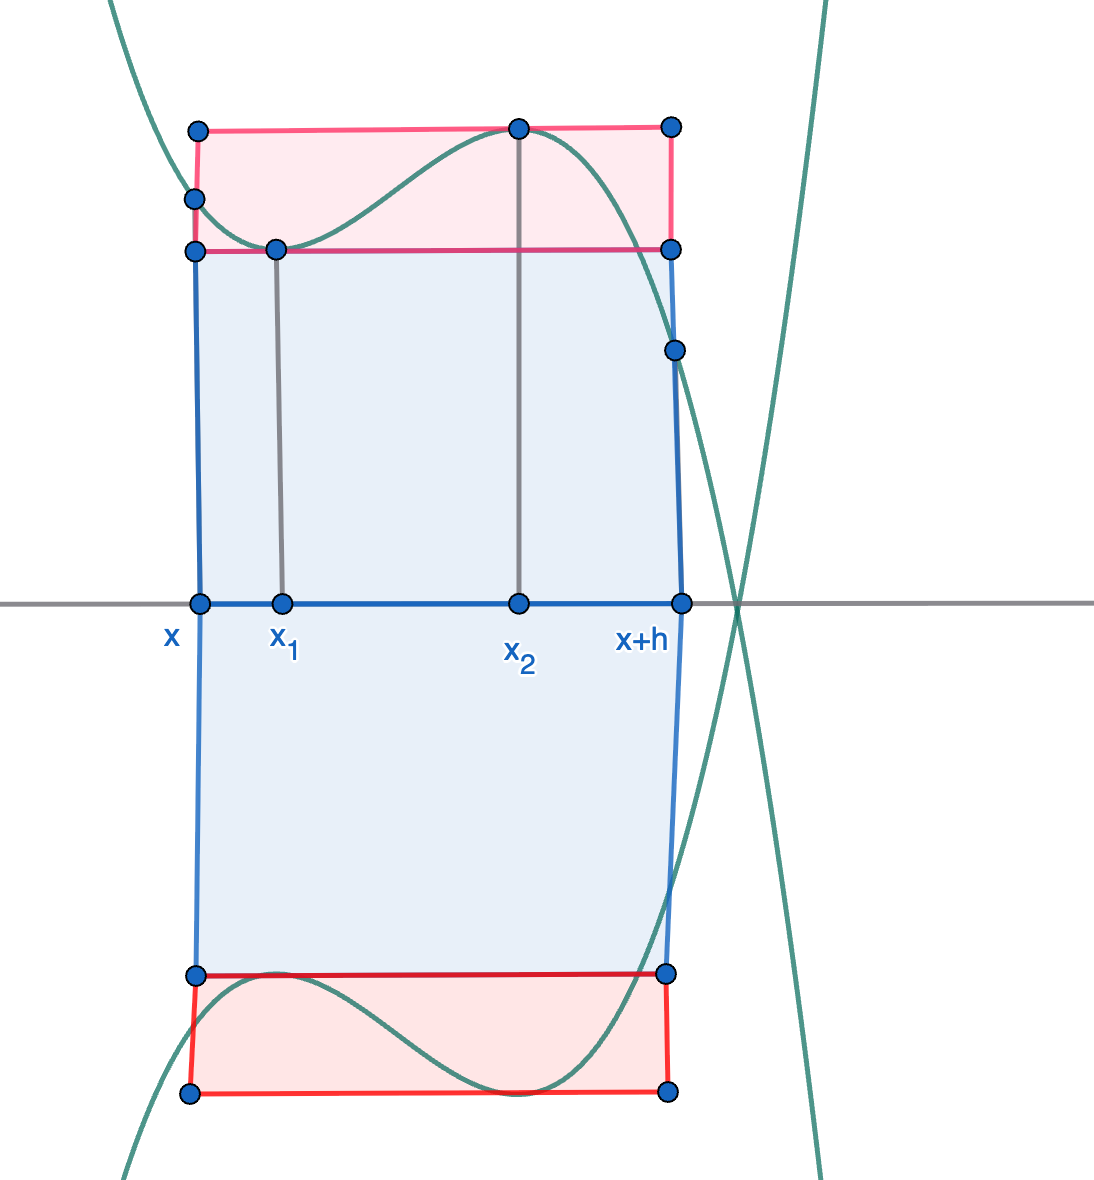
\includegraphics[scale=0.4]{skitser/omdrejningslegeme.png}
\end{figure}

Vi kigger igen på et interval $x$ til $x+h$,
hvor vi er interesserede i volumnet af det omdrejningslegeme,
der fremkommer, når grafen roteres omkring $x$-aksen.
Vi går igen ud fra, at en funktion $V(x)$ giver volumen af omdrejningslegemet
indtil $x$, så volumnet i intervallet er $V=V(x+h)-V(x)$.
Vi antager, at $V(x)$ er differentiabel i intervallet.

Derudover kan vi approksimere volumnet. Som på skitsen
så må der i intervallet være et lokalt minimum og maksimum.
Volumnet må være større eller lig med volumnet af den cylinder,
der har radius $f(x_1)$ og længde $h$, hvis volumen er udtrykt ved:

$$
    V_{min}=h \cdot \pi f(x_1)^2
$$

Omvendt kan volumnet maksimalt være lig med volumnet af cylinderen,
der har højde $f(x_2)$ og længde $h$, hvis areal er:

$$
    V_{max}=h \cdot \pi f(x_2)^2
$$

Nu kan vi opstille følgende ulighed:

$$
h \cdot \pi f(x_1)^2
\leq
V(x+h)-V(x)
\leq
h \cdot \pi f(x_2)^2
$$

Vi deler med $h$:

$$
\pi f(x_1)^2
\leq
\frac{V(x+h)-V(x)}{h}
\leq
 \pi f(x_2)^2
$$

Så lader vi $h \rightarrow 0$, deraf:

\begin{align*}
     x_1 &\rightarrow x \\
    x_2 &\rightarrow x \\
    f(x_1) &\rightarrow f(x) \\
    f(x_2) &\rightarrow f(x) \\
    \frac{V(x+h)-V(x)}{h} &\rightarrow V'(x)
\end{align*}

Så vi får følgende udtryk:

$$
\pi f(x)^2
\leq
V'(x)
\leq
 \pi f(x)^2
$$

Som betyder, at:

$$
V'(x)
=\pi f(x)^2
$$

Vi har vist, at volumen funktionen for det omdrejningslegeme, der fremkommer,
kan findes ved at tage integralet af ovenstående udtryk.

\end{proofw}
